\documentclass{article}
\usepackage[utf8]{inputenc}
\usepackage{physics}
\usepackage{listings}
\usepackage{graphicx}
\usepackage{flexisym}

%%%%%%%%%%%%%%%%%%%%%%%%%%%%%%%%%%
\documentclass[10pt, a4paper, twoside]{article}
\usepackage[margin=1in,bindingoffset=5.5mm,heightrounded]{geometry}
\usepackage[T1]{fontenc}
\usepackage{indentfirst}
%\vspace*{36 pt}
\title{Applied Mathematics TW324 Assignment 05}
\author{https://github.com/BhekimpiloNdhlela/TW324NumericalMethods \\ \\ Bhekimpilo Ndhlela (18998712)}
\date{04 May 2018}
\begin{document}
\maketitle
\pagebreak
\section*{Python Library Source Code Question 1 and 2: }
\begin{lstlisting}[language=Python]
def composite_midpoint(f, m, a=0.0, b=1.0):
    h = (b-a)/m
    return h*sum([f((a+h/2.0) + i*h) for i in xrange(0, m)])

def composite_trapezium(f, m, a=0.0, b=1.0):
    h = (b - a) / m
    return h/2.0*(f(a)+f(b)+2*sum([f(a+i*h) for i in xrange(1,m)]))

def composite_simpson(f, m, a=0.0, b=1.0):
    sum = float(f(a) + f(b))
    h   = (b-a) / (2*m)
    oddSum, evenSum = 0.0, 0.0
    for i in range(1, m):
        oddSum += f(2 * h * i + a)
    sum += oddSum * 2
    for i in range(1,m+1):
        evenSum += f(h * (-1 + 2 * i) + a)
    sum += evenSum * 4
    return sum * h / 3

def debug(abs_err_cm, abs_err_ct, abs_err_cs, debug=True):
    if debug == True:
        print("DEBUG MODE STATUS = <ON>")
        print("Composite Midpoint\tComposite trapezium\tComposite_Simpson")
        for m, t, s in zip(abs_err_cm, abs_err_ct, abs_err_cs):
                print "{:.20f}     ".format(m), \
                      "{:.20f}     ".format(t), \
                      "{:.20f}     ".format(s)

def plot_abs_errs(abs_err_cm, abs_err_ct, abs_err_cs):
    plt.title("|xc-x| of: The Composite Midpoint, Simpson & Trapezium Methods"\
              "against h")
    plt.ylabel("Composite[Midpoint vs Simpson vs Trapezium]")
    plt.xlabel("Number of Points")
    plt.xscale('log')
    plt.yscale('log')
    plt.plot(M, abs_err_cm, 'k-', label="Composite Midpoint")
    plt.plot(M, abs_err_ct, 'r-', label="Composite Trapezium")
    plt.plot(M, abs_err_cs, 'b-', label="Composite Simpson")
    plt.legend(bbox_to_anchor=(.65, .9))
    plt.show()
\end{lstlisting}
\pagebreak


\section*{Question 1}
\subsection*{Python Client Source Code For question 1}
\begin{lstlisting}[language=Python]
from numpy import (abs, array, linspace)
from scipy import (integrate, special)
import matplotlib.pyplot as plt
from math import exp
f = lambda x : exp(x)
I = integrate.quad(f, 0.0, 1.0)[0]; M = linspace(11, 101, 10)
abs_err_cm = [abs(composite_midpoint(f, int(m)) - I) for m in M]
abs_err_ct = [abs(composite_trapezium(f, int(m))- I) for m in M]
abs_err_cs = [abs(composite_simpson(f, int(m))  - I) for m in M]
debug(abs_err_cm, abs_err_ct, abs_err_cs)
plot_abs_errs(abs_err_cm, abs_err_ct, abs_err_cs)
\end{lstlisting}

\begin{figure}[h!]
  \centering
  \begin{subfigure}{\linewidth}
    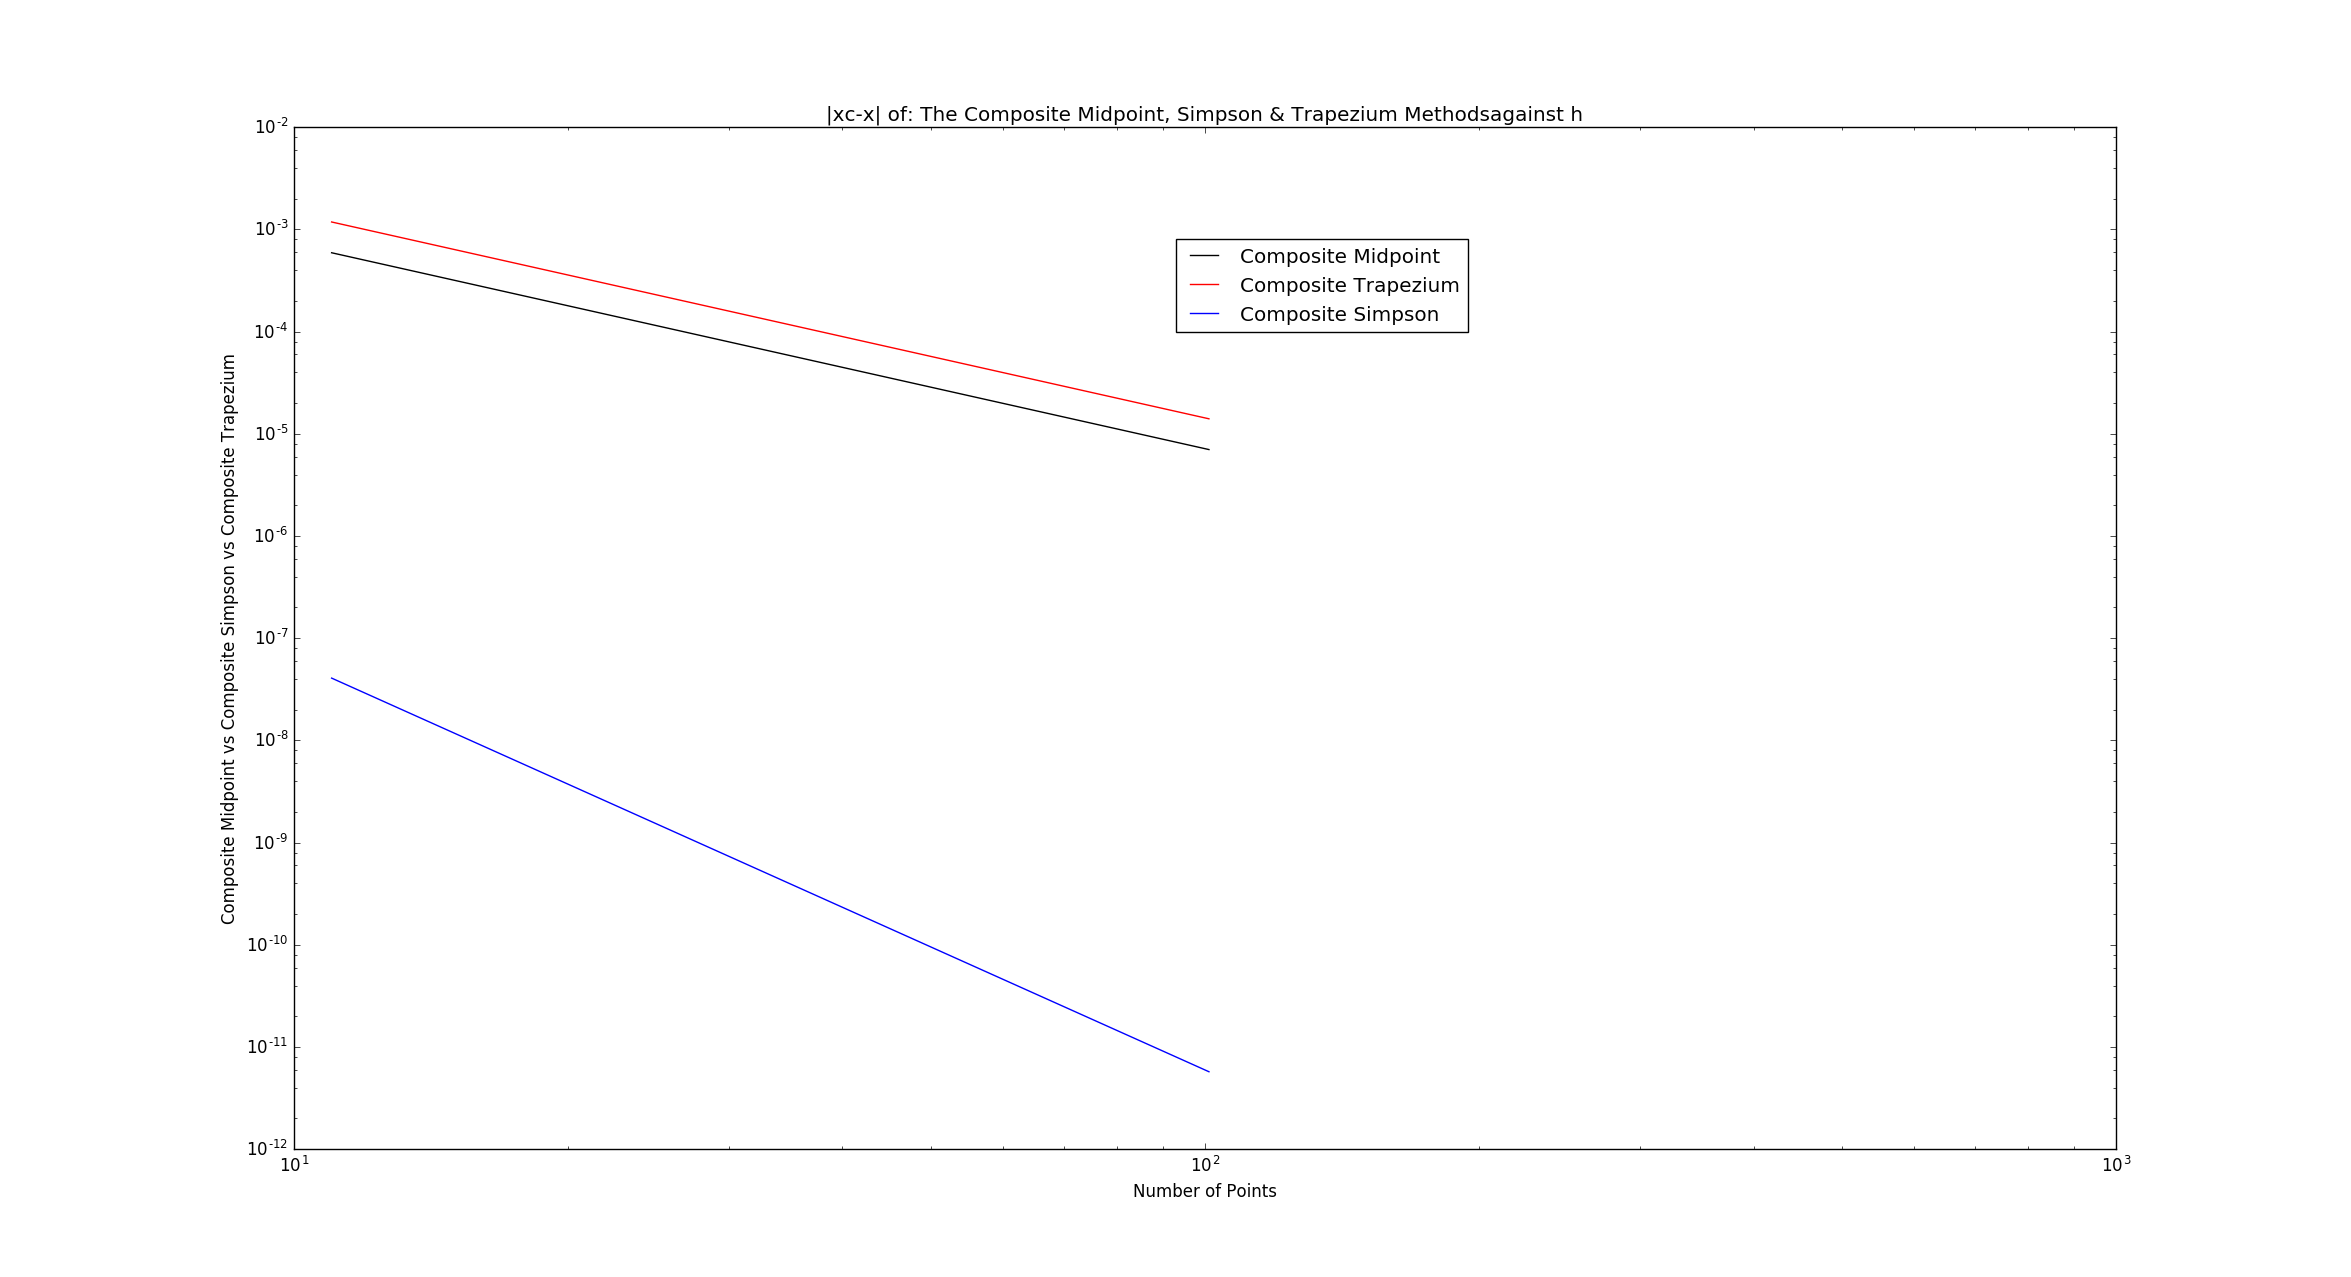
\includegraphics[width=\linewidth]{question1.png}
    \caption{|xc-x| of $ I = \int_{0}^{1} e^x dx $ comparing The Composite Midpoint, Simpson & Trapezium Methods against h}
  \end{subfigure}
\end{figure}
\textbf{\\Comparison Results:\\
For question 4 (Assignment 4) The absolute errors $| x_c - x|$ of the Midpoint, Simpson's and 
the Trapezium method are increasing as h increases and for question 1 (Assignment 5) the Absolute
error $| x_c - x|$ for Composite (Midpoint, Trapezium and Simpson) methods are decreasing as the number
of pallets/ points used increases.}
\pagebreak


\section*{Question 2}
\subsection*{Python Client Source Code For question 2}
\begin{lstlisting}[language=Python]
import matplotlib.pyplot as plt
from math import (exp, pi, sin)
from scipy import (integrate, special)
from numpy import (abs, array, linspace)
f = lambda x : exp(sin(2 * pi * x))
I = integrate.quad(f, 0.0, 1.0)[0]; M = linspace(3, 19, 5)
abs_err_cm = [abs(composite_midpoint(f, int(m)) - I) for m in M]
abs_err_ct = [abs(composite_trapezium(f, int(m)) - I) for m in M]
abs_err_cs = [abs(composite_simpson(f, int(m)) - I) for m in M]
debug(abs_err_cm, abs_err_ct, abs_err_cs, debug=True)
plot_abs_errs(abs_err_cm, abs_err_ct, abs_err_cs)
\end{lstlisting}
\begin{figure}[h!]
  \centering
  \begin{subfigure}{\linewidth}
    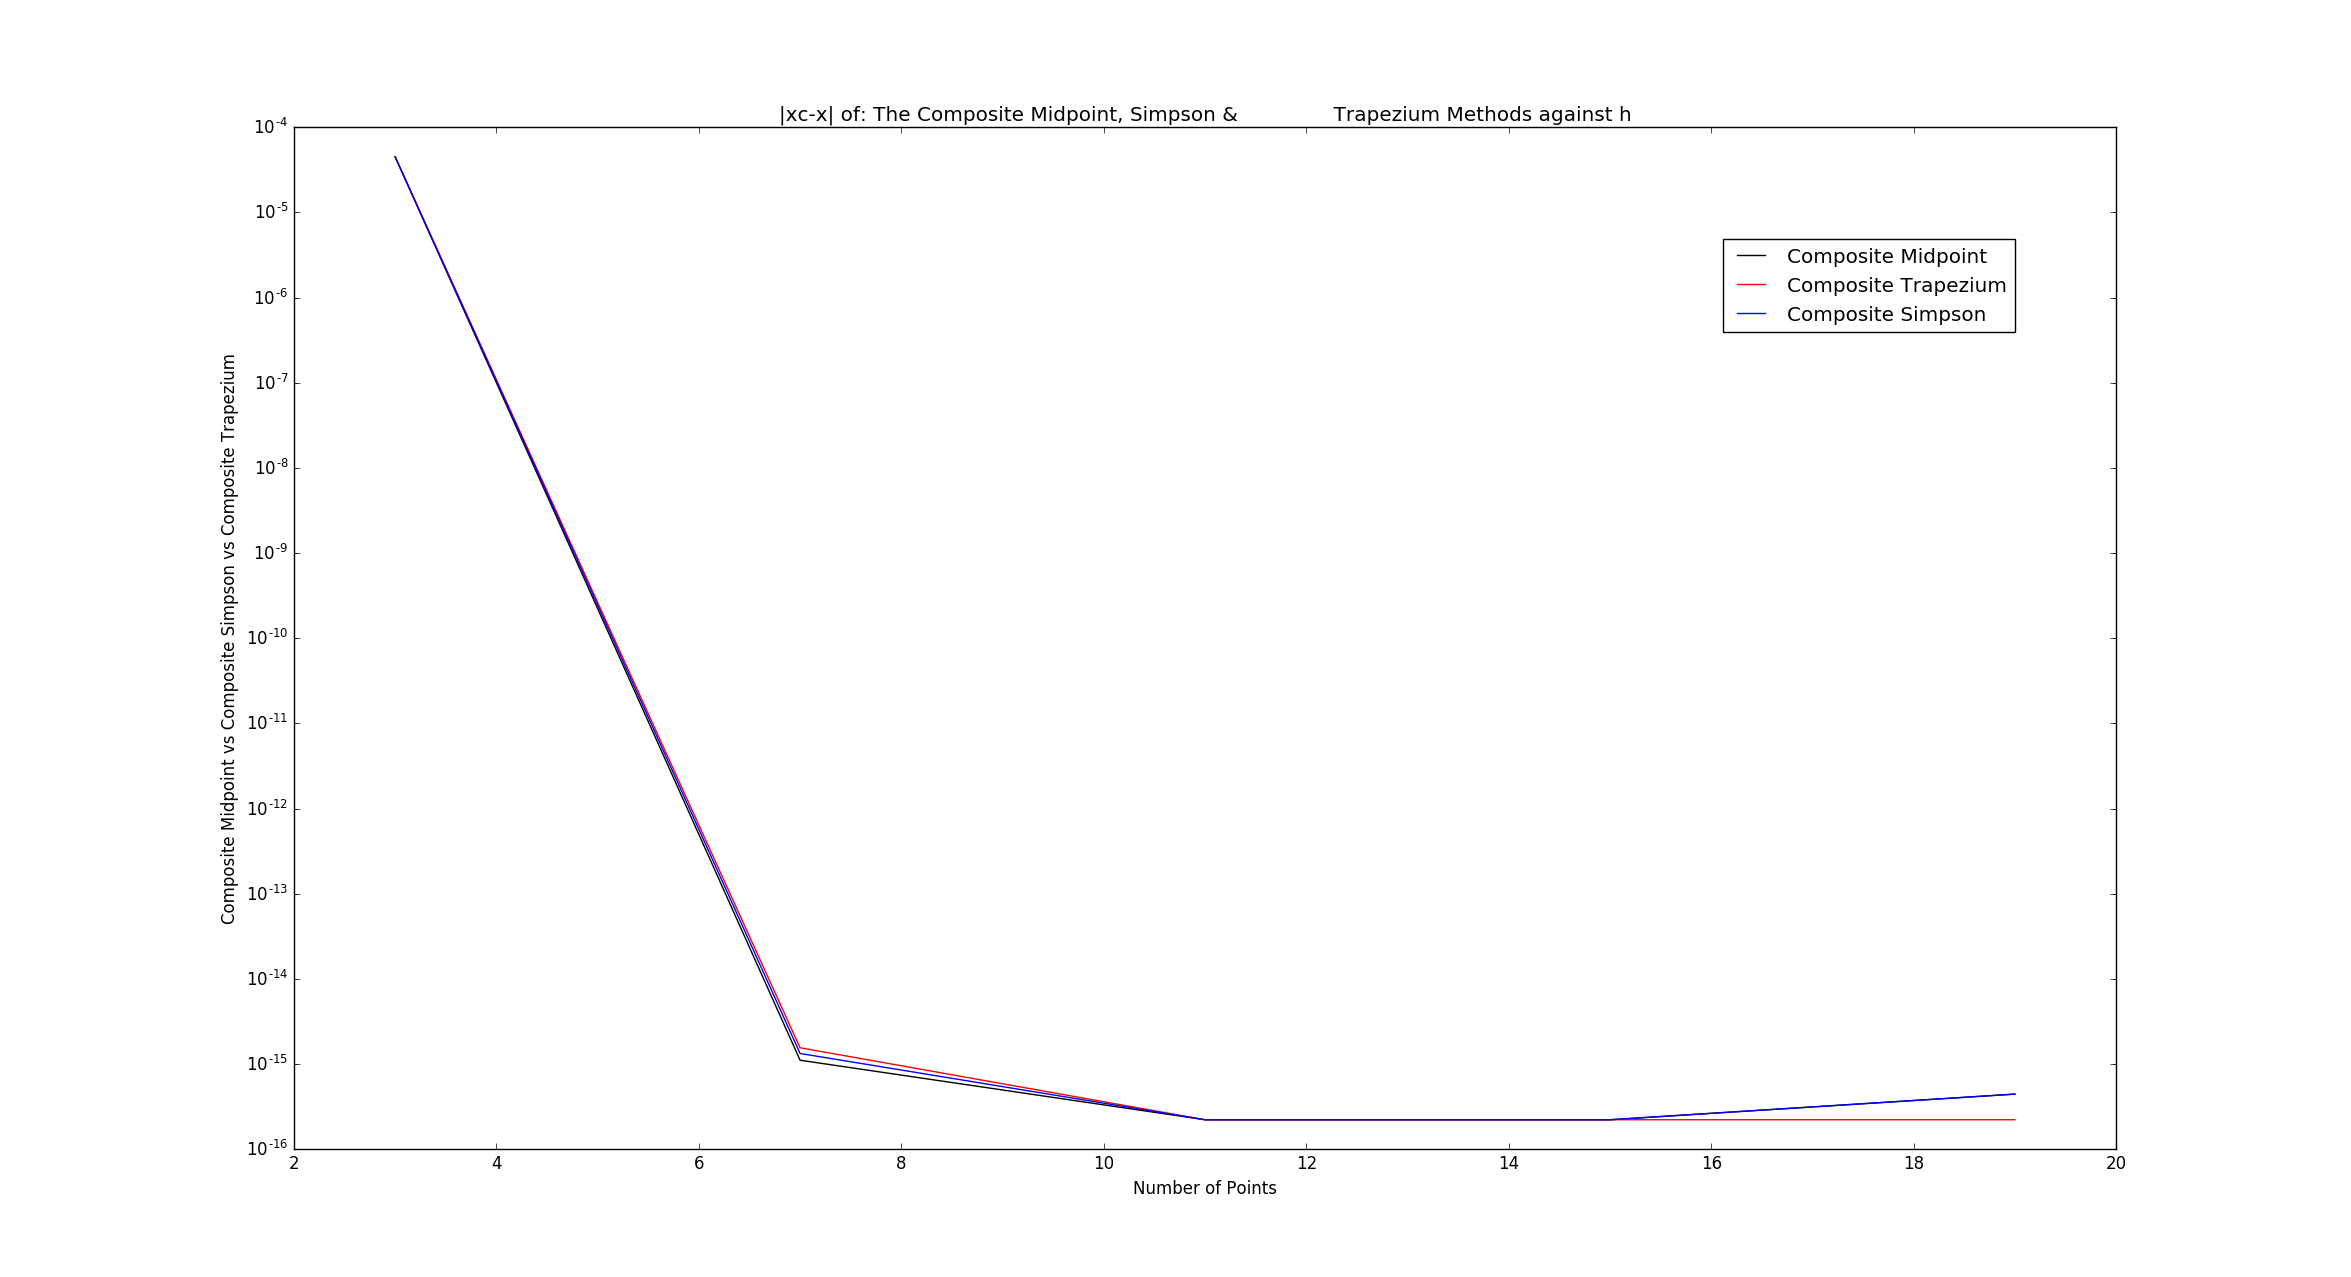
\includegraphics[width=\linewidth]{question2.png}
    \caption{|xc-x| of $ I = \int_{0}^{1} e^{\sin(2 \pi x)} dx $ comparing The Composite Midpoint, Simpson & Trapezium Methods against h}
  \end{subfigure}
\end{figure}
\textbf{Comparison Results: for question 1 the Absolute
error $| x_c - x|$ for Composite Midpoint, Trapezium and Simpson methods are decreasing linearly with a constant gradient as the number of pallets/ points used increases. However, for question 2 as the number of pallets/ points used increases the error function decrease with linearly for but with a different gradient. Also for question 2 the vertical distance between the error functions is very small. It is also evident that as $n \approx 15 $ the composite Simpson and Midpoint start increasing but the composite trapezium remains constant}
\pagebreak

\section*{Question 3}
\subsection*{Python Source Code For question 3}
\begin{lstlisting}[language=Python]
def question_b(f0, f1, debug=True):
    r0, r1 = romberg(f0, 0.0, 1.0, 5), romberg(f1, 0.0, 1.0, 5)
    if debug == True:
        print "Debug Mode: [ON] Question 3(b)\n"
        debug_on(r0, "Romberg results For Function in Problem 1 :")
        debug_on(r1, "\nRomberg results For Function in Problem 2 :")
    return r0, r1

def question_c(r0, r1, f0, f1, N=5, debug=True):
    I0, I1 = integrate.quad(f0, 0.0, 1.0)[0], integrate.quad(f1, 0.0, 1.0)[0]
    e0, e1 = romberg_abs_error(r0, I0), romberg_abs_error(r1, I1)
    if debug == True:
        print "Debug Mode: [ON] Question 3(b)\n"
        debug_on(e0, "Romberg Error results For Function in Problem 1 :")
        debug_on(e1, "\nRomberg Error results For Function in Problem 2 :")
    return e0, e1

def romberg_abs_error(r, I):
    e = zeros((len(r), len(r)))
    for i in xrange(0, len(e)):
        for j in xrange(0, len(e)):
            if r[i][j] == 0.0: continue
            else: e[i][j] = abs(r[i][j] - I)
    return e

def debug_on(matrix, debug_message):
    print(debug_message)
    for row in matrix: print "[",
        for element in row: print "{:.15f}   ".format(element),
        print("]")

if __name__ == "__main__":
    from romberg import romberg
    import matplotlib.pyplot as plt
    from math import (exp, pi, sin)
    from scipy import (integrate, special)
    from numpy import (abs, array, linspace, zeros)

    f0, f1 = lambda x : exp(x), lambda x : exp(sin(2 * pi * x))
    r0, r1 = question_b(f0, f1)
    e0, e1 = question_c(r0, r1, f0, f1)
\end{lstlisting}

\pagebreak
\textbf{\\ \\ \\ 5x5 Romberg Matrix for the approximation of : $ I = \int_{0}^{1} e^x dx $\\ \\}
         $R_{5x5}$ = \begin{bmatrix}1.859140914229523 & 0.000000000000000 & 0.000000000000000 & 0.000000000000000 & 0.000000000000000\\
                                    1.753931092464825 & 1.718861151876593 & 0.000000000000000 & 0.000000000000000 & 0.000000000000000\\
                                    1.727221904557517 & 1.718318841921747 & 1.718282687924758 & 0.000000000000000 & 0.000000000000000\\
                                    1.720518592164302 & 1.718284154699897 & 1.718281842218440 & 1.718281828794531 & 0.000000000000000\\
                                    1.718841128579994 & 1.718281974051892 & 1.718281828675358 & 1.718281828460389 & 1.718281828459078 \end{bmatrix}
                                   
                                   
                                    
\textbf{\\ \\ \\ 5x5 Romberg Matrix for the approximation of : $ I = \int_{0}^{1} e^{\sin(2 \pi x)} dx $\\ \\ }
         $R_{5x5}$ = \begin{bmatrix}1.000000000000000 & 0.000000000000000 & 0.000000000000000 & 0.000000000000000 & 0.000000000000000\\
                                    1.000000000000000 & 1.000000000000000 & 0.000000000000000 & 0.000000000000000 & 0.000000000000000\\
                                    1.271540317407622 & 1.362053756543496 & 1.386190673646396 & 0.000000000000000 & 0.000000000000000\\
                                    1.266066076964489 & 1.264241330150111 & 1.257720501723885 & 1.255681292645750 & 0.000000000000000\\
                                    1.266065877752008 & 1.266065811347848 & 1.266187443427697 & 1.266321839327758 & 1.266363566961805 \end{bmatrix}


\textbf{\\ \\ \\ Absolute Error for : $ I = \int_{0}^{1} e^x dx $\\ \\}
         $R_{5x5}$ = \begin{bmatrix}0.140859085770477 & 0.000000000000000 & 0.000000000000000 & 0.000000000000000 & 0.000000000000000\\
                                    0.035649264005780 & 0.000579323417548 & 0.000000000000000 & 0.000000000000000 & 0.000000000000000\\
                                    0.008940076098471 & 0.000037013462702 & 0.000000859465712 & 0.000000000000000 & 0.000000000000000\\
                                    0.002236763705256 & 0.000002326240852 & 0.000000013759395 & 0.000000000335485 & 0.000000000000000\\
                                    0.000559300120949 & 0.000000145592847 & 0.000000000216313 & 0.000000000001343 & 0.000000000000033\end{bmatrix}

\textbf{\\ \\ \\ Absolute Error for : $ I = \int_{0}^{1} e^{\sin(2 \pi x)} dx $\\ \\}
         $R_{5x5}$ = \begin{bmatrix}0.266065877752008 & 0.000000000000000 & 0.000000000000000 & 0.000000000000000 & 0.000000000000000\\
                                    0.266065877752008 & 0.266065877752008 & 0.000000000000000 & 0.000000000000000 & 0.000000000000000\\
                                    0.005474439655614 & 0.095987878791488 & 0.120124795894387 & 0.000000000000000 & 0.000000000000000\\
                                    0.000000199212481 & 0.001824547601897 & 0.008345376028123 & 0.010384585106258 & 0.000000000000000\\
                                    0.000000000000000 & 0.000000066404160 & 0.000121565675689 & 0.000255961575750 & 0.000297689209797 \end{bmatrix}
                                    
\textbf{\\ \\ \\ \\ Comenting on the most accurate entry:\\ The most accurate entry should have the smallest Absolute Error $|x_c - x|$ in the Romberg Matrix there for It is evident that the most accurate entry for: \\  $ I = \int_{0}^{1} e^x dx $ is the $R_{55}$  entry.\\  $ I = \int_{0}^{1} e^{\sin(2 \pi x)} dx $ is the $R_{51}$ entry .  }
\pagebreak

\section*{Question 4}
\subsection*{Python Source Code For Question 4: }
\begin{lstlisting}[language=Python]
def computing_with_gauss(f, n=5.0):
    X, C = gauss(int(n), [0, 1])
    return  sum([float(c) * f(float(x)) for x, c in zip(X, C)])

def computing_with_fejer(f, n=5.0):
    X, C = fejer(int(n), [0, 1])
    return sum([float(c) * f(float(x)) for x, c in zip(X, C)])

if __name__ == "__main__":
    from math import exp
    from fejer import fejer
    from gauss import gauss
    from scipy import integrate

    f = lambda x : exp(x)
    I = integrate.quad(f, 0.0, 1.0)[0]
    abs_err = lambda xc, x : abs(xc - x)

    gauss_I, fejer_I = computing_with_gauss(f),  computing_with_fejer(f)
    abs_err_gauss, abs_err_fejer = abs_err(gauss_I, I), abs_err(fejer_I, I)

    debug = True
    if debug == True:
        print("Debug Mode Status: <ON>")
        print("exact_I = {:.20f}".format(float(I)))
        print"gauss_I = {:.20f}".format(float(gauss_I)), "\t",
        print"abs_err_gauss = {:.20f}".format(float(abs_err_gauss))
        print"fejer_I = {:.20f}".format(float(fejer_I)), "\t",
        print"abs_err_fejer = {:.20f}".format(float(abs_err_fejer))
\end{lstlisting}
 
\textbf{\\Remark/ Comparisons:\\ Given or Knowing that the Exact Integral $= 1.71828182845904531284$. Considering the Table of results below, I can thus conclude on my findings:\\ Gauss Legendre is more accurate compared to the Fejer's-Approximation This is evident because the Gauss Legendre's Absolute Error $|X_c - X|$ is smaller compared to the Fejer's-Approximation. However, if one is to compare the Gauss Legendre Method against the Results of the Romberg Method in problem 3 one can conclude by saying that the Romberg's Method is more accurate compared to the Gauss Legendre's Method, this is evident because the Absolute Error $|X_c - X| = R_{55} = 0.00000000000003286260 $($R_{55}$ being the best entry) vs the  Gauss Legendre's Absolute error  $ = |X_c - X| = 00000000000891331453$ which is not as good as the $R_{55} $ entry of Romberg's Matrix. There for for this specific problem (Problem 1) Romberg's Method is more accurate compared to the Gauss Legendre's Method.\\ \\ }
\begin{center}
\begin{tabular}{ |c|c|c| } 
 \hline \hline
                      & Approximation Results  & Absolute Error \\ 
\hline \hline       
 Gauss-Legendre       & 1.71828182845013199831 & 0.00000000000891331453 \\ 
 \hline
 Fejer-Approximations & 1.71828193633821713071 & 0.00000010787917181787 \\ 
 \hline
\end{tabular}
\end{center}


\pagebreak

\section*{Question 5}
\subsection*{Python Source Code For Question 5: }
\begin{lstlisting}[language=Python]
def gauss_legendre(n=5.0):
    X, C = gauss(5, [-1, 1])
    f = lambda x : exp(x) / sqrt(1 - x**2)
    return sum([f(float(x)) * float(c) for x, c in zip(X, C)])

def gauss_chebyshev(n=5.0):
    X = [cos(((2.0 * i - 1) * pi) / (2 * n)) for i in xrange(1, int(n + 1))]
    return (pi * (sum([exp(x) for x in X]))) / n

if __name__ == "__main__":
    from scipy import (integrate, special)
    from math import (sqrt, exp, cos, pi)
    from gauss import gauss

    exact_integral = integrate.quad(lambda x : exp(x)/sqrt(1-x**2),-1,1)[0]
    gauss_chebyshev, gause_legendre = gauss_chebyshev(), gauss_legendre()

    debug = True
    if debug == True:
        print("Debug Mode Status: <ON>")
        print("Exact Integral  = {:.20f}".format(float(exact_integral)))
        print("Gauss Chebyshev = {:.20f}".format(abs(float(gauss_chebyshev)\
                                          - float(exact_integral))))
        print("Gauss Legendre  = {:.20f}".format(abs(float(gause_legendre)\
                                          - float(exact_integral))))
\end{lstlisting}

\textbf{\\ \\ \\ Results: \\ By the Python Scipy Integrate function/ method the Exact Integral to the problem to 20 dp is $ = 3.97746326050611820335$ \\From the results in the Table the Gauss Chebyshev Method is more accurate compared to the Gauss Legendre method because it is evident from the absolute error that the Gauss Legendre method has the biggest Absolute Error $|x_c - x|$. \\ This may be caused by the fact that Gauss Chebyshev only considers the Numerator $e^x$ when approximating the Integral but the Gauss Legendre consider both the Numerator and the denominator when approximating the integral ($\frac{e^x}{\sqrt{1 - x^2}}$)\\ \\}
 \begin{center}
\begin{tabular}{ |c|c|c| } 
 \hline \hline
                      & Approximation Results  & Absolute Error \\ 
\hline \hline       
 Gauss-Legendre       & 3.48653636094816832269 & 0.49092689955794988066 \\ 
 \hline
 Gauss-Chebyshev      & 3.97746325877669448801 & 0.00000000172942371535 \\ 
 \hline
\end{tabular}
\end{center}

\pagebreak

\section*{Question 6}
\subsection*{Python Source Code For both Question 6a.) and 6b.): }
\begin{lstlisting}[language=Python]
def question_a(f, n, w0, I, G=9.81, C2=1.0/1000.0):
    T = linspace(0.0, 10.0, n)
    h = 10.0/float(n) # step size
    w = zeros(n+1, dtype=float)
    w[0] = w0
    for i in xrange(1, n+1):
        w[i] = w[i-1] + h * f(w[i-1])
    return abs(w[-1] - I)

def explicit_trapezium(f, n, w0, I, G=9.81, C2=1.0/1000.0):
    T = linspace(0.0, 10.0, n)
    h = 10.0/float(n) # step size
    w, wt = zeros(n+1, dtype=float), zeros(n+1, dtype=float)
    w[0] = w0
    for i in xrange(1, n+1):
        wt[i] = w[i-1] + h * f(w[i-1])
        w[i]  = w[i-1] + h * f(wt[i-1] + h/2.0 * f(wt[i]))
    return abs(w[-1] - I)

def explicit_midpoint(f, n, w0, I, G=9.81, C2=1.0/1000.0):
    T = linspace(0.0, 10.0, n)
    h = 10.0/float(n) # step size
    w, wt = zeros(n+1, dtype=float), zeros(n+1, dtype=float)
    w[0] = w0
    for i in xrange(1, n+1):
        wt[i] = w[i-1] + 0.5 * h * f(w[i-1])
        w[i]  = w[i-1] + h * f(wt[i])
    return abs(w[-1] - I)

def debug_on(errors, N, I, debug_message, debug=False):
    if debug == False:
        pass
    else:
        print "\n************************************************************"
        print "Method Used: ", debug_message
        print "The Exact Value I = {:.20f}".format(float(I))
        for error, n in zip(errors, N):
            print "@ n = ", n, "the abs_err = {:.20f}".format(error)
        print "************************************************************"

def plot_computed_error(N, abs_err_0, abs_err_1=None, abs_err_2=None):
    plt.ylabel("n = number of points")
    plt.xlabel("h = step size)")
    plt.xscale('log'); plt.yscale('log')
    if abs_err_1 == None and abs_err_2 == None:
        plt.title("6(b.) Absolute Error of Euler's method with n = 10, 100 1000")
        plt.plot(N, abs_err_0, 'k-')
        plt.show()
    else:
        plt.title("(6a.) Absolute Error of Euler's, Explicit Midpoint"\
                   "and Explicit Trapezium methods with n = 10, 100 1000")
        plt.plot(N, abs_err_0, 'k-', label="Error Euler's Method")
        plt.plot(N, abs_err_1, 'b-', label="Error Explicit Midpoint Method")
        plt.plot(N, abs_err_2, 'r-', label="Error Explicit Trapezium Method")
        plt.legend(bbox_to_anchor=(1.0, 1.0))
        plt.show()

if __name__ == "__main__":
    from numpy import (linspace, array, zeros)
    from scipy import (integrate, special)
    import matplotlib.pyplot as plt
    from math import (sqrt, tanh)

    f = lambda t : 9.81 - (1.0/1000.0) * (t**2)
    I = sqrt(9.81/(1.0/1000.0)) * tanh(10. * sqrt(9.81*(1.0/1000.0)))
    N = [10, 100, 1000]

    # get absolute error using Euler's meth6od
    abs_errors_eulr = [question_a(f, n, 0.0, I) for n in N]
    debug_on(abs_errors_eulr, N, I, "Euler's Method")

    # get absolute error using explicit trapezium method
    abs_errors_trap = [explicit_trapezium(f, n, 0.0, I) for n in N]
    debug_on(abs_errors_trap, N, I, "Explicit Trapezium Method")

    # get absolute error using explicit midpoint method
    abs_errors_midp = [explicit_midpoint(f, n, 0.0, I) for n in N]
    debug_on(abs_errors_midp, N, I, "Explicit Midpoint Method")

    # plot the error for question 6(a.)
    plot_computed_error(N, abs_errors_eulr)
    # plot the error for question 6(a.) and 6(b.) on the same cartesion plane
    plot_computed_error(N, abs_errors_eulr, abs_errors_midp, abs_errors_trap)
\end{lstlisting}
\textbf{\\ \\ \\ Commenting On Graphs Bellow (Figure 4): \\ The Absolute $|x_c - x|$ of the Euler's, Explicit Midpoint and the Explicit Trapezium Method are all decreasing as $h$ the stwep size is increased. However the Explicit Trapezium Method is the most accurate, followed by the Explicit Midpoint and lastly the Euler's Method. Also it is good to note that the Explicit Trapezium and Explicit Midpoint Methods competing as h increases. }
\pagebreak
\begin{figure}[h!]
  \centering
  \begin{subfigure}{\linewidth}
    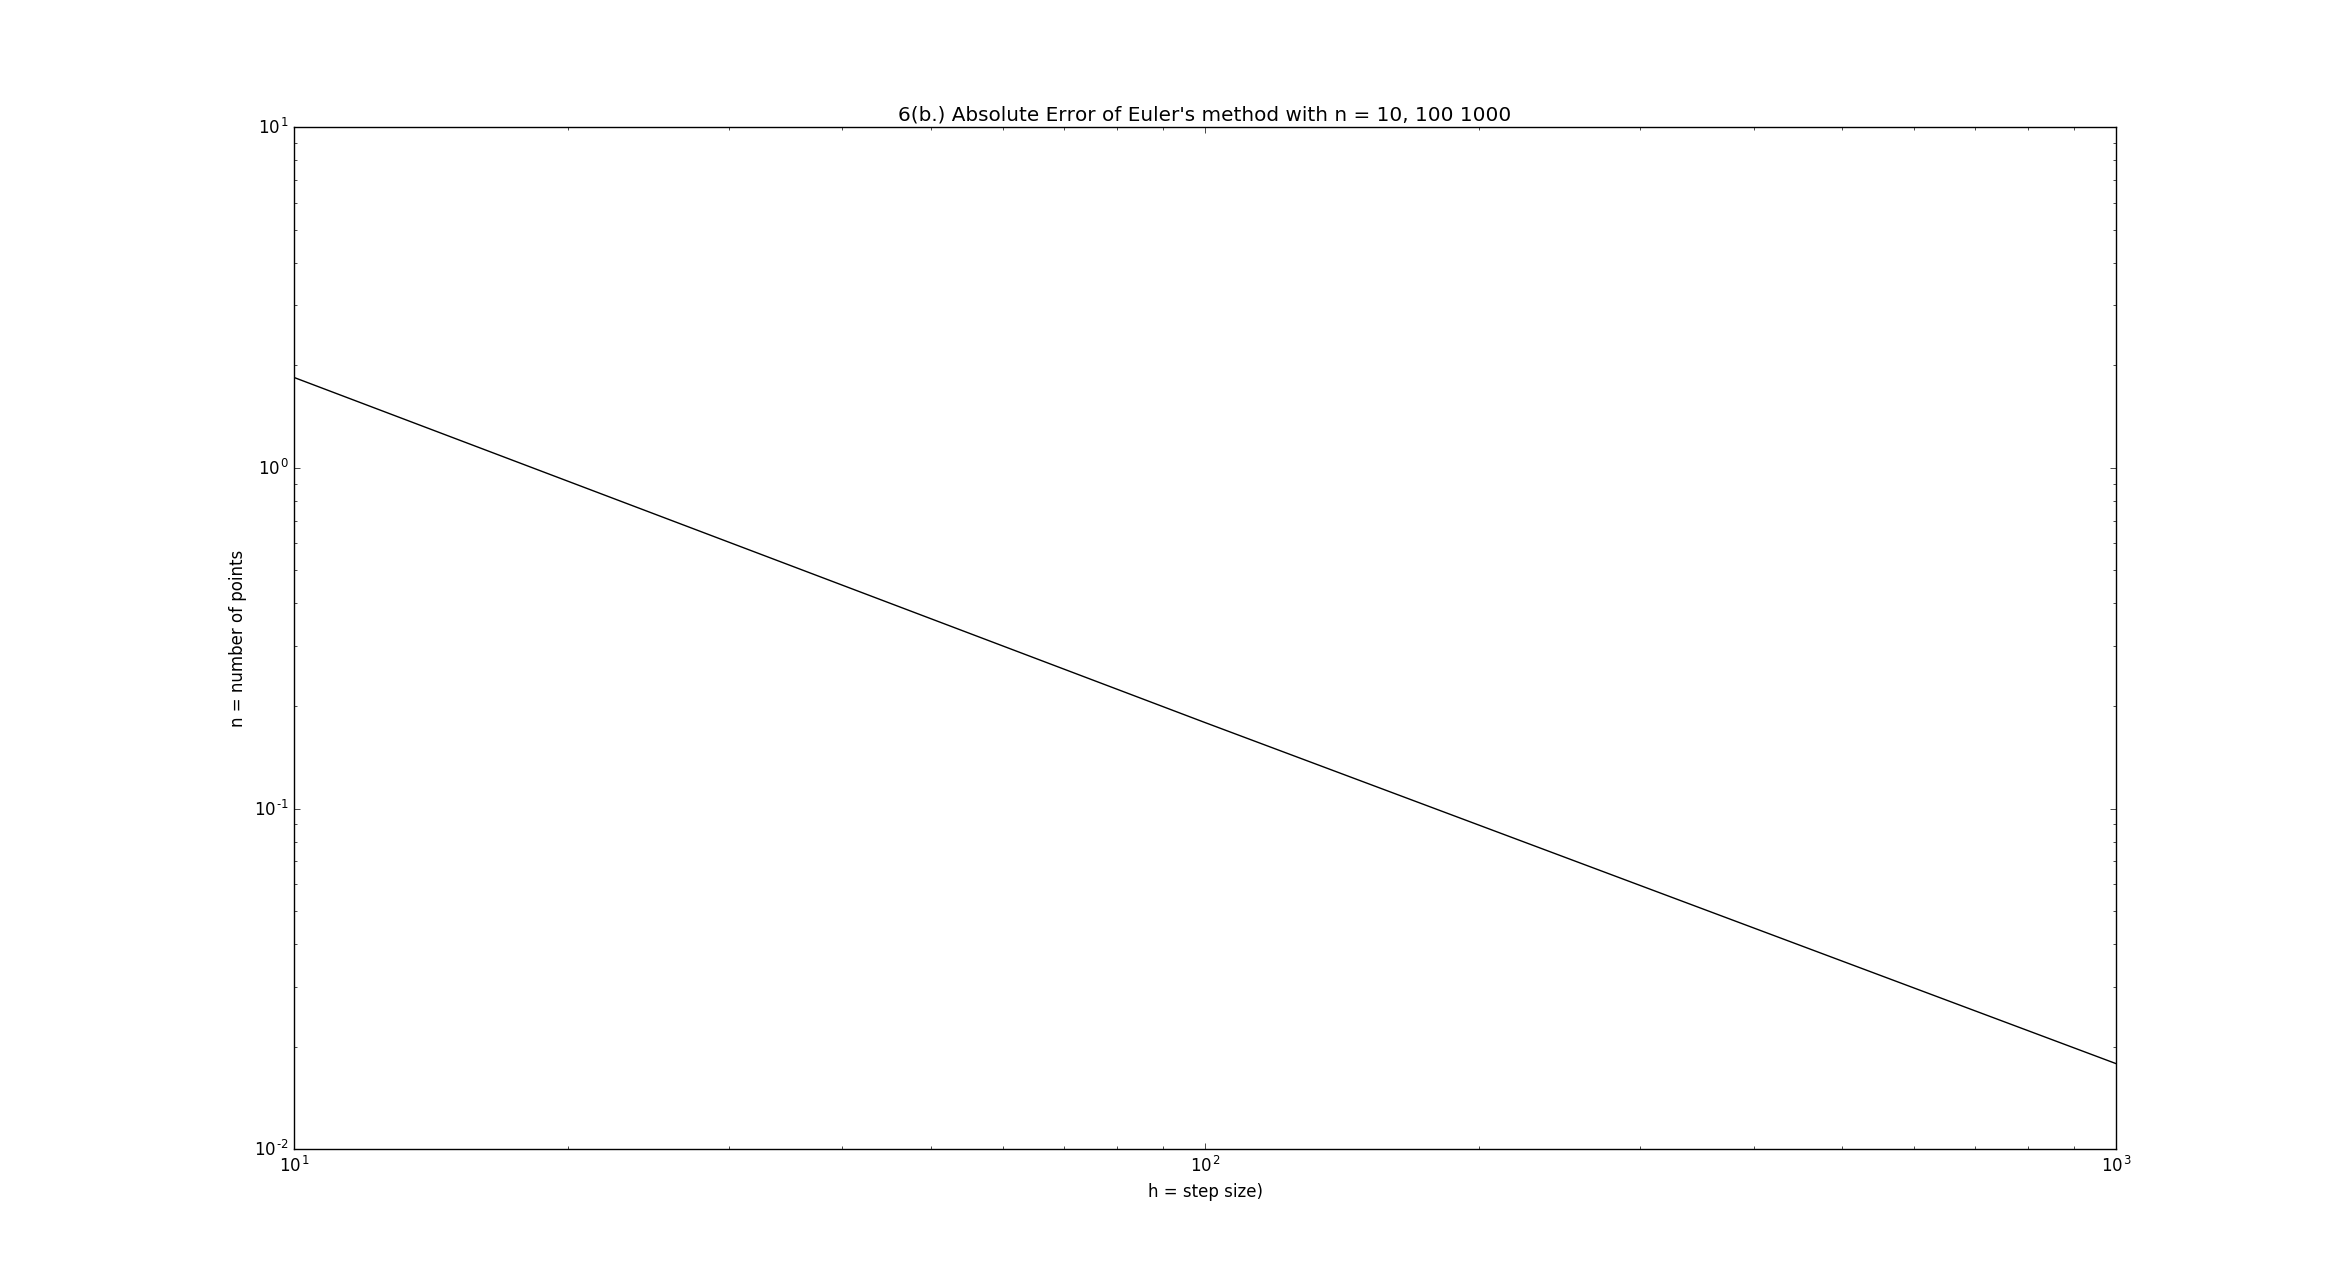
\includegraphics[width=\linewidth]{question6a.png}
    \caption{$|X_c - X|$ of Euler's method on $\frac{dV}{dt} = 9.81 - C_2v^2$, $y_0 = w_0 = 0$ with n = 10, 100 1000}
  \end{subfigure}
\end{figure}
%\pagebreak

\begin{figure}[h!]
  \centering
  \begin{subfigure}{\linewidth}
    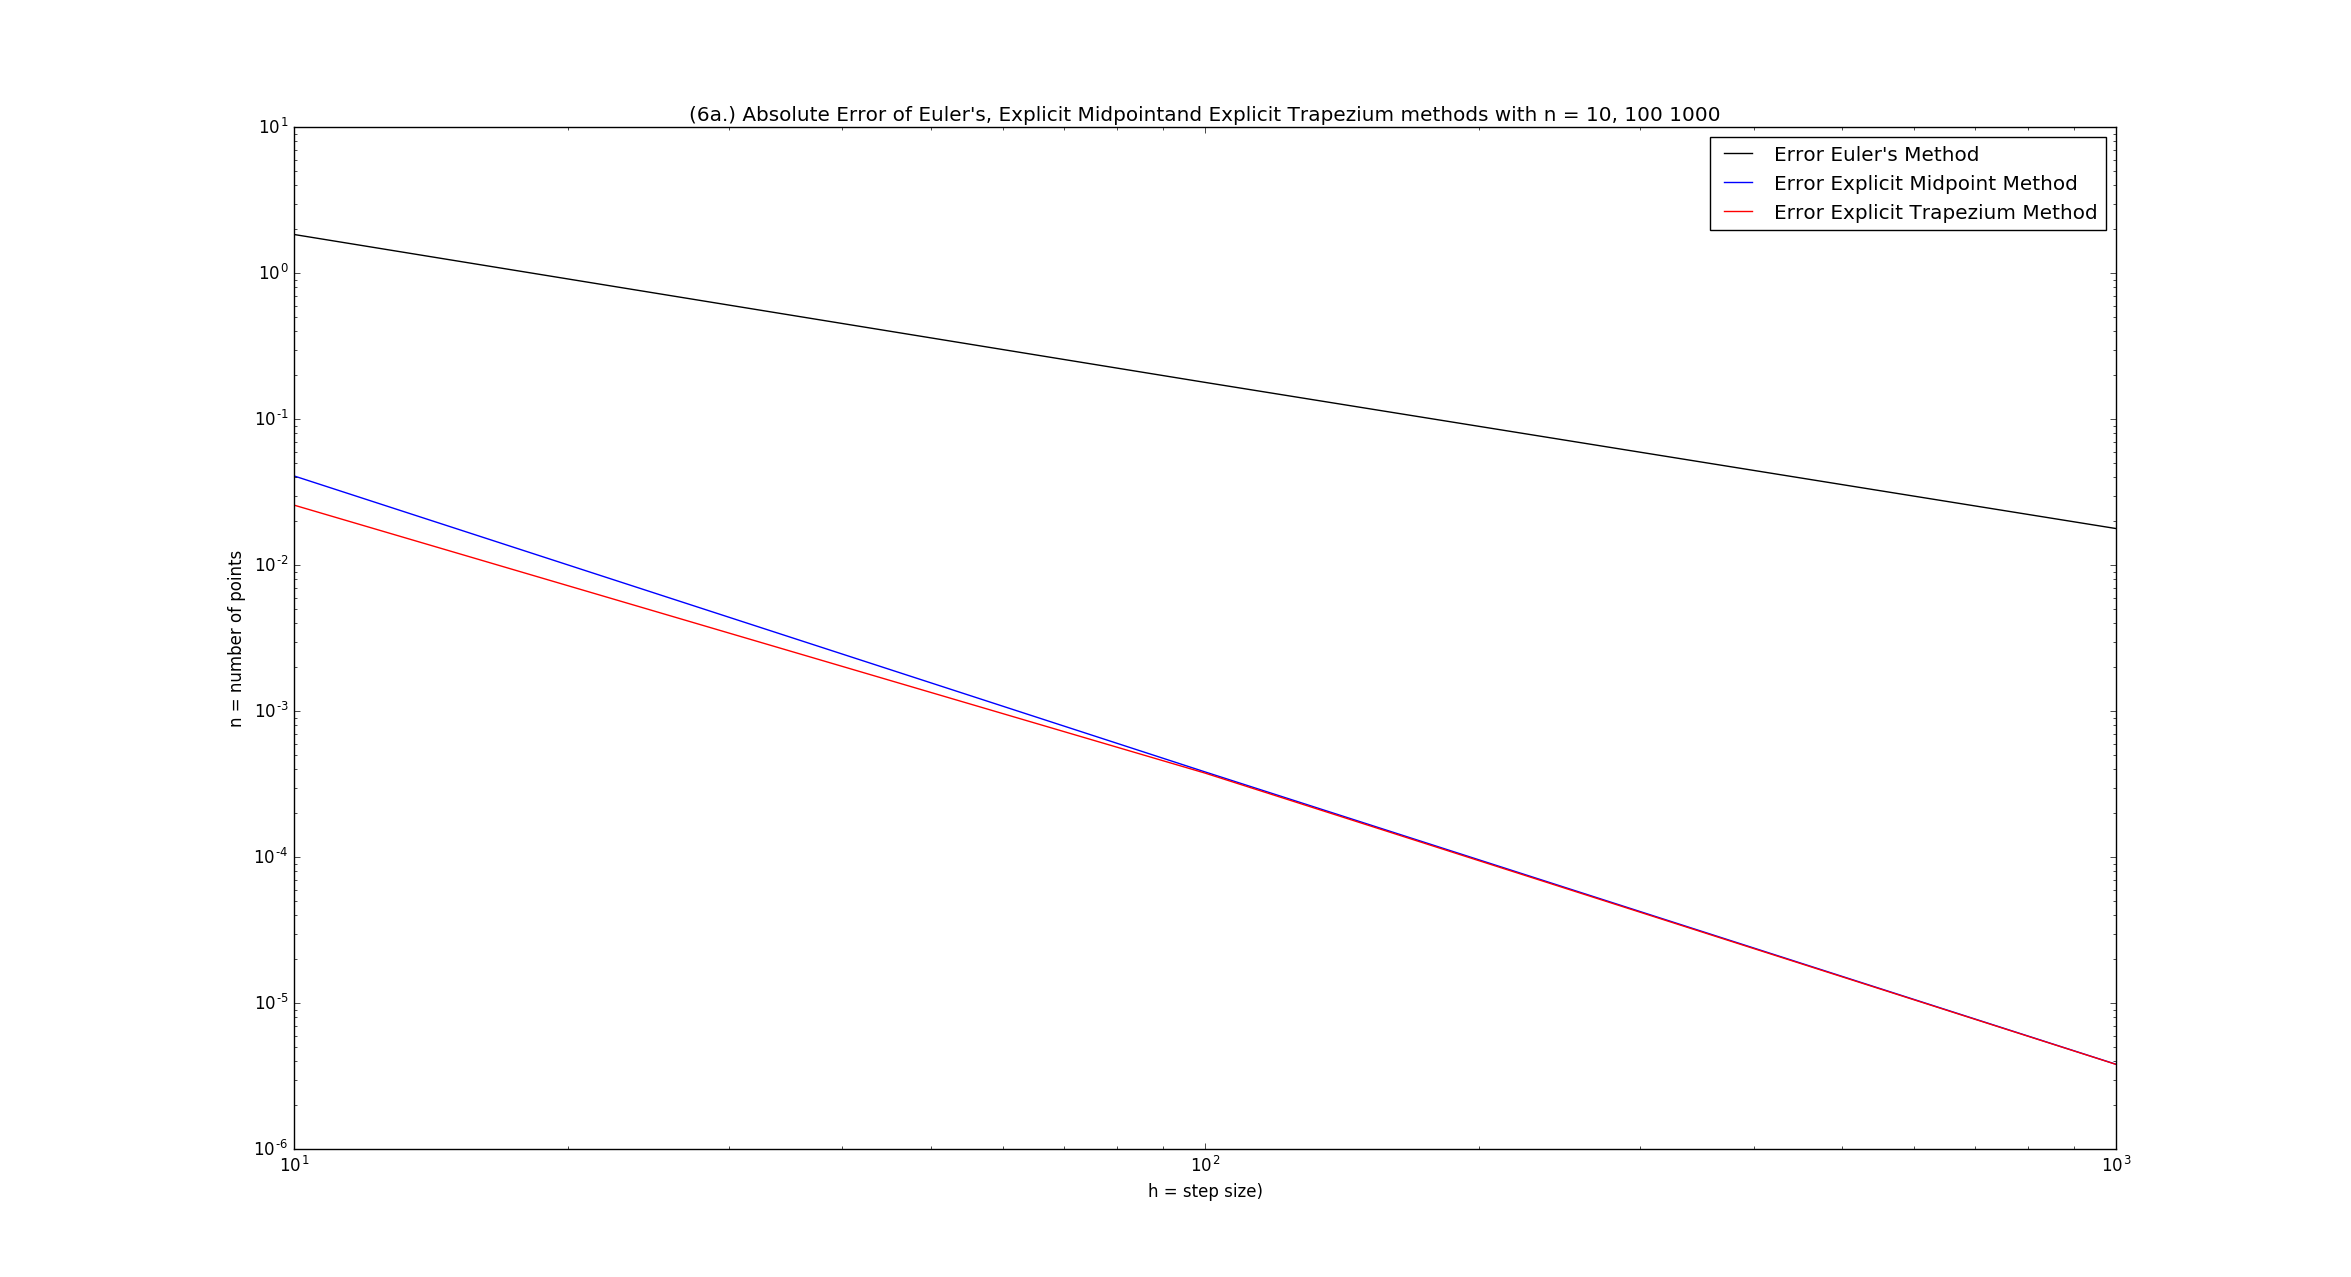
\includegraphics[width=\linewidth]{question6b.png}
    \caption{$|X_c - X|$ of Euler's, Expl Trapezium and Expl explicit trapezium and explicit
midpointexplicit trapezium and explicit
midpointMidpoint method on $\frac{dV}{dt} = 9.81 - C_2v^2$, $y_0 = w_0 = 0$ with n = 10, 100 1000}
  \end{subfigure}
\end{figure}
\pagebreak
\end{document}



